\documentclass[a4paper, 11pt]{article}

%set margins
\usepackage[left=2.5cm, top=2.5cm, right=2.5cm, bottom=2.5cm]{geometry}

%package for equations
\usepackage{amsmath}

% disables indentation
\parindent=0pt 

%set space between two paragraphs
\setlength{\parskip}{1em}

%package for figures
\usepackage{graphicx}
\graphicspath{ {./Figures/} }

%package for captions
\usepackage{caption}

\title{\bf{CoBRA segmentor}}
\author{}
\date{}


\begin{document}	
\maketitle
\vspace{-7em}

\section{Application interface}
The CoBRA segmentor application was developped to facilitate segmentation of images within the CoBRA project (Cow Behaviour Recording and Analysis). The main interface of the CoBRA segmentor is shown in figure \ref{fig:application_main_view} and contains three parts. The left side displays the image one is currently annotating, both the annotated objects, as well as the annotated masks can be visualised. On the right top of the application, one can find a part devoted to the class of each object, for each declared class, a radiobutton will be provided enabling easy selection of the right category for each object. These buttons are conservative and will keep the class of the last declared object as the default class for newly declared object, thereby increasing annotation performance. On the right bottom of the application one can find an area devoted to all declared objects and masks, this part can be used to rename objects and masks (double left click) or modify them after declaration. Also this part of the application offers the opportunity to hide all declared masks, making the whole imag again visible.

\begin{figure}[h]
	\centering
	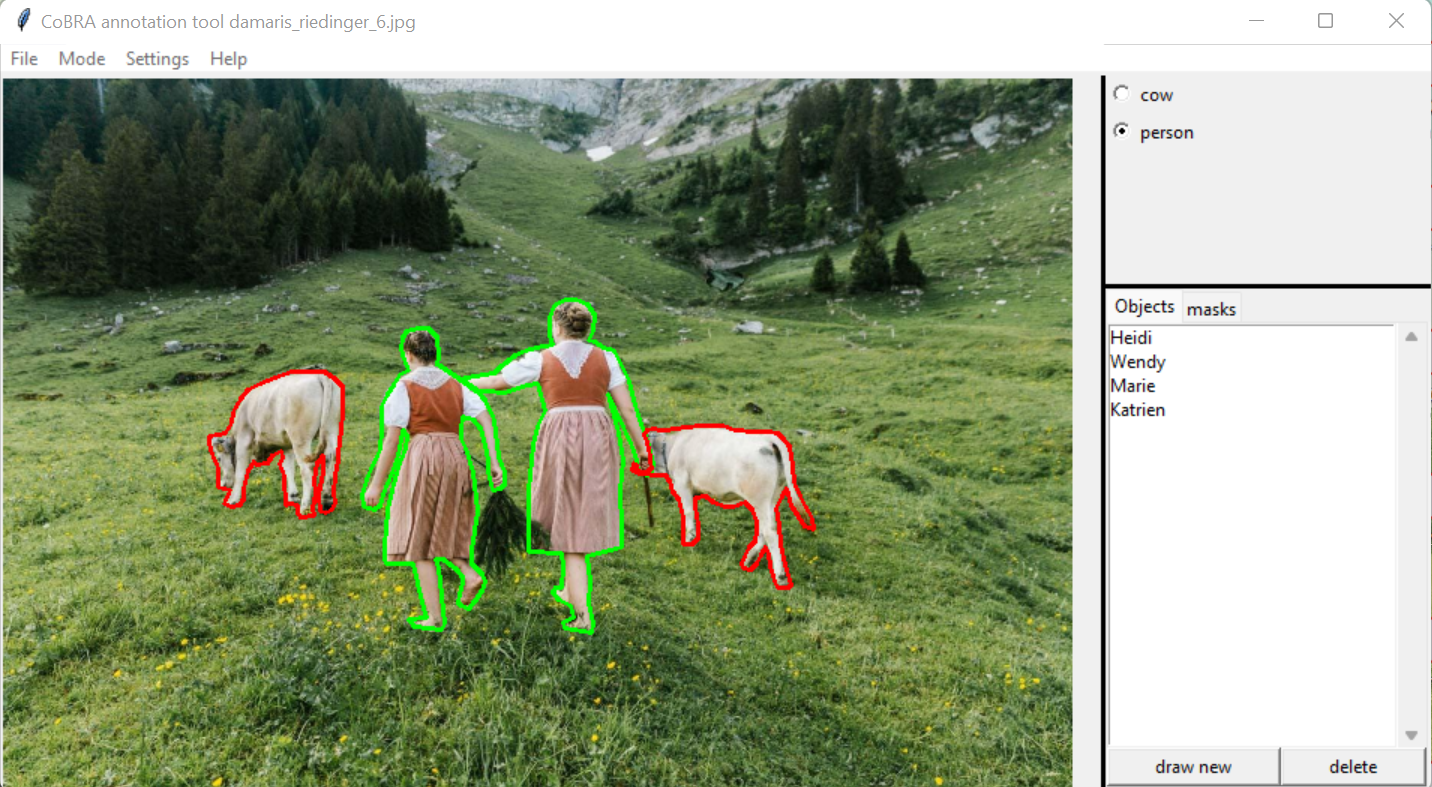
\includegraphics[width=\textwidth]{application_main_view}
	\captionsetup{width=0.8\textwidth}
	\caption{Main interface of the application.}
	\label{fig:application_main_view}
\end{figure}

Apart from the main window, multiple subwindows are available, increasing the functionality of the software. One of these interfaces is the category manager , displayed in figure \ref{fig:category manager}. In this manager, one can add new object categories, rename existing categories and, if necessary, delete categories. It is recommended to be extremely careful with deleting categories, since this will lead to the irreversible loss of all objects belonging to the deleted category.

\begin{figure}[h!]
	\centering
	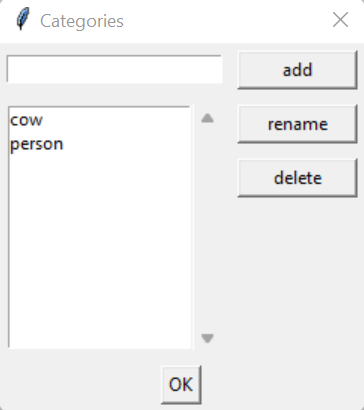
\includegraphics[width=0.5\textwidth]{category_manager}
	\captionsetup{width=0.5\textwidth}
	\caption{Category manager.}
	\label{fig:category manager}
\end{figure}

When categories are added in the category manager, they are assigned automatically a color. These automatically selected colors are chosen with the aim of an optimal contrast between objects of different categories. If one wants however to change the color of a certain category, the color manager is available (figure \ref{fig:color manager}), enabling to specify a custom color for each category by means of RGB color encoding.

\begin{figure}[h!]
	\centering
	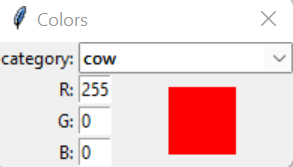
\includegraphics[width=0.3\textwidth]{color_manager}
	\captionsetup{width=0.3\textwidth}
	\caption{color manager.}
	\label{fig:color manager}
\end{figure}


\section{Common annotation workflow}

\begin{enumerate}
	\item Open an image (Ctrl + O)
	\item Annotate an object by drawing an appropriate bbox/convex hull/segment around it. One can move all vertices of the bbox/convex hull/segment or split edges
	\item Choose the appropriate class of the object. If the class of the current object is the same as the class of the previous object, the right class will be automatically selected
	\item Confirm the object (Enter)
	\item Repeat steps 2 - 4 until all objects on the image are annotated
	\item Save the annotations (CTRl + S)
	\item Open the next (F8) or previous (F7) image
	\item Repeat steps 2 - 6 until all the images in the dataset are annotated
	\item Export a dataset (F5)
\end{enumerate}

\section{Mouse events}


\begin{tabular}{ p{2cm} p{14cm}}
	left click & Draw a new point. If one clicks on a yet existing point, the point will be re-activated and can be moved to a more appropriate position. If one clicks on an edge, the edge will be splitted and a new point will appear on the place were one clicked. One can move the active point as long as one holds down the left mouse button. Once the left mouse button is released, the point will be fixed on it's current position\\ 
	scroll & Zoom in/out \\  
	right click & Move the image (only available if the image doesn't fit on the window)     
\end{tabular}


\section{Shortcuts}


\begin{tabular}{ p{2cm} p{13cm}}
	Enter & Confirm object\\ 
	Ctrl + O & Open image\\  
	Ctrl + Z & Undo last change\\  
	Ctrl + S & Save annotations\\ 
	Ctrl + I & Import images\\
	F1 & Open help\\ 
	F5 & Export dataset\\ 
	F7 & Open previous image\\ 
	F8 & Open next image\\  
\end{tabular}

\end{document}